% !TEX root = BachelorBookletMain.tex

\chapter{Introduction}
Shrouded mirror is an experimental experience, where the player sees the world through the eyes of a neural network. The player moves through an environment, collects beacons and avoids enemies. Each type of entity emits a unique audio signal, creating a distinctive soundscape.
\begin{figure}[hbt]
\centering
    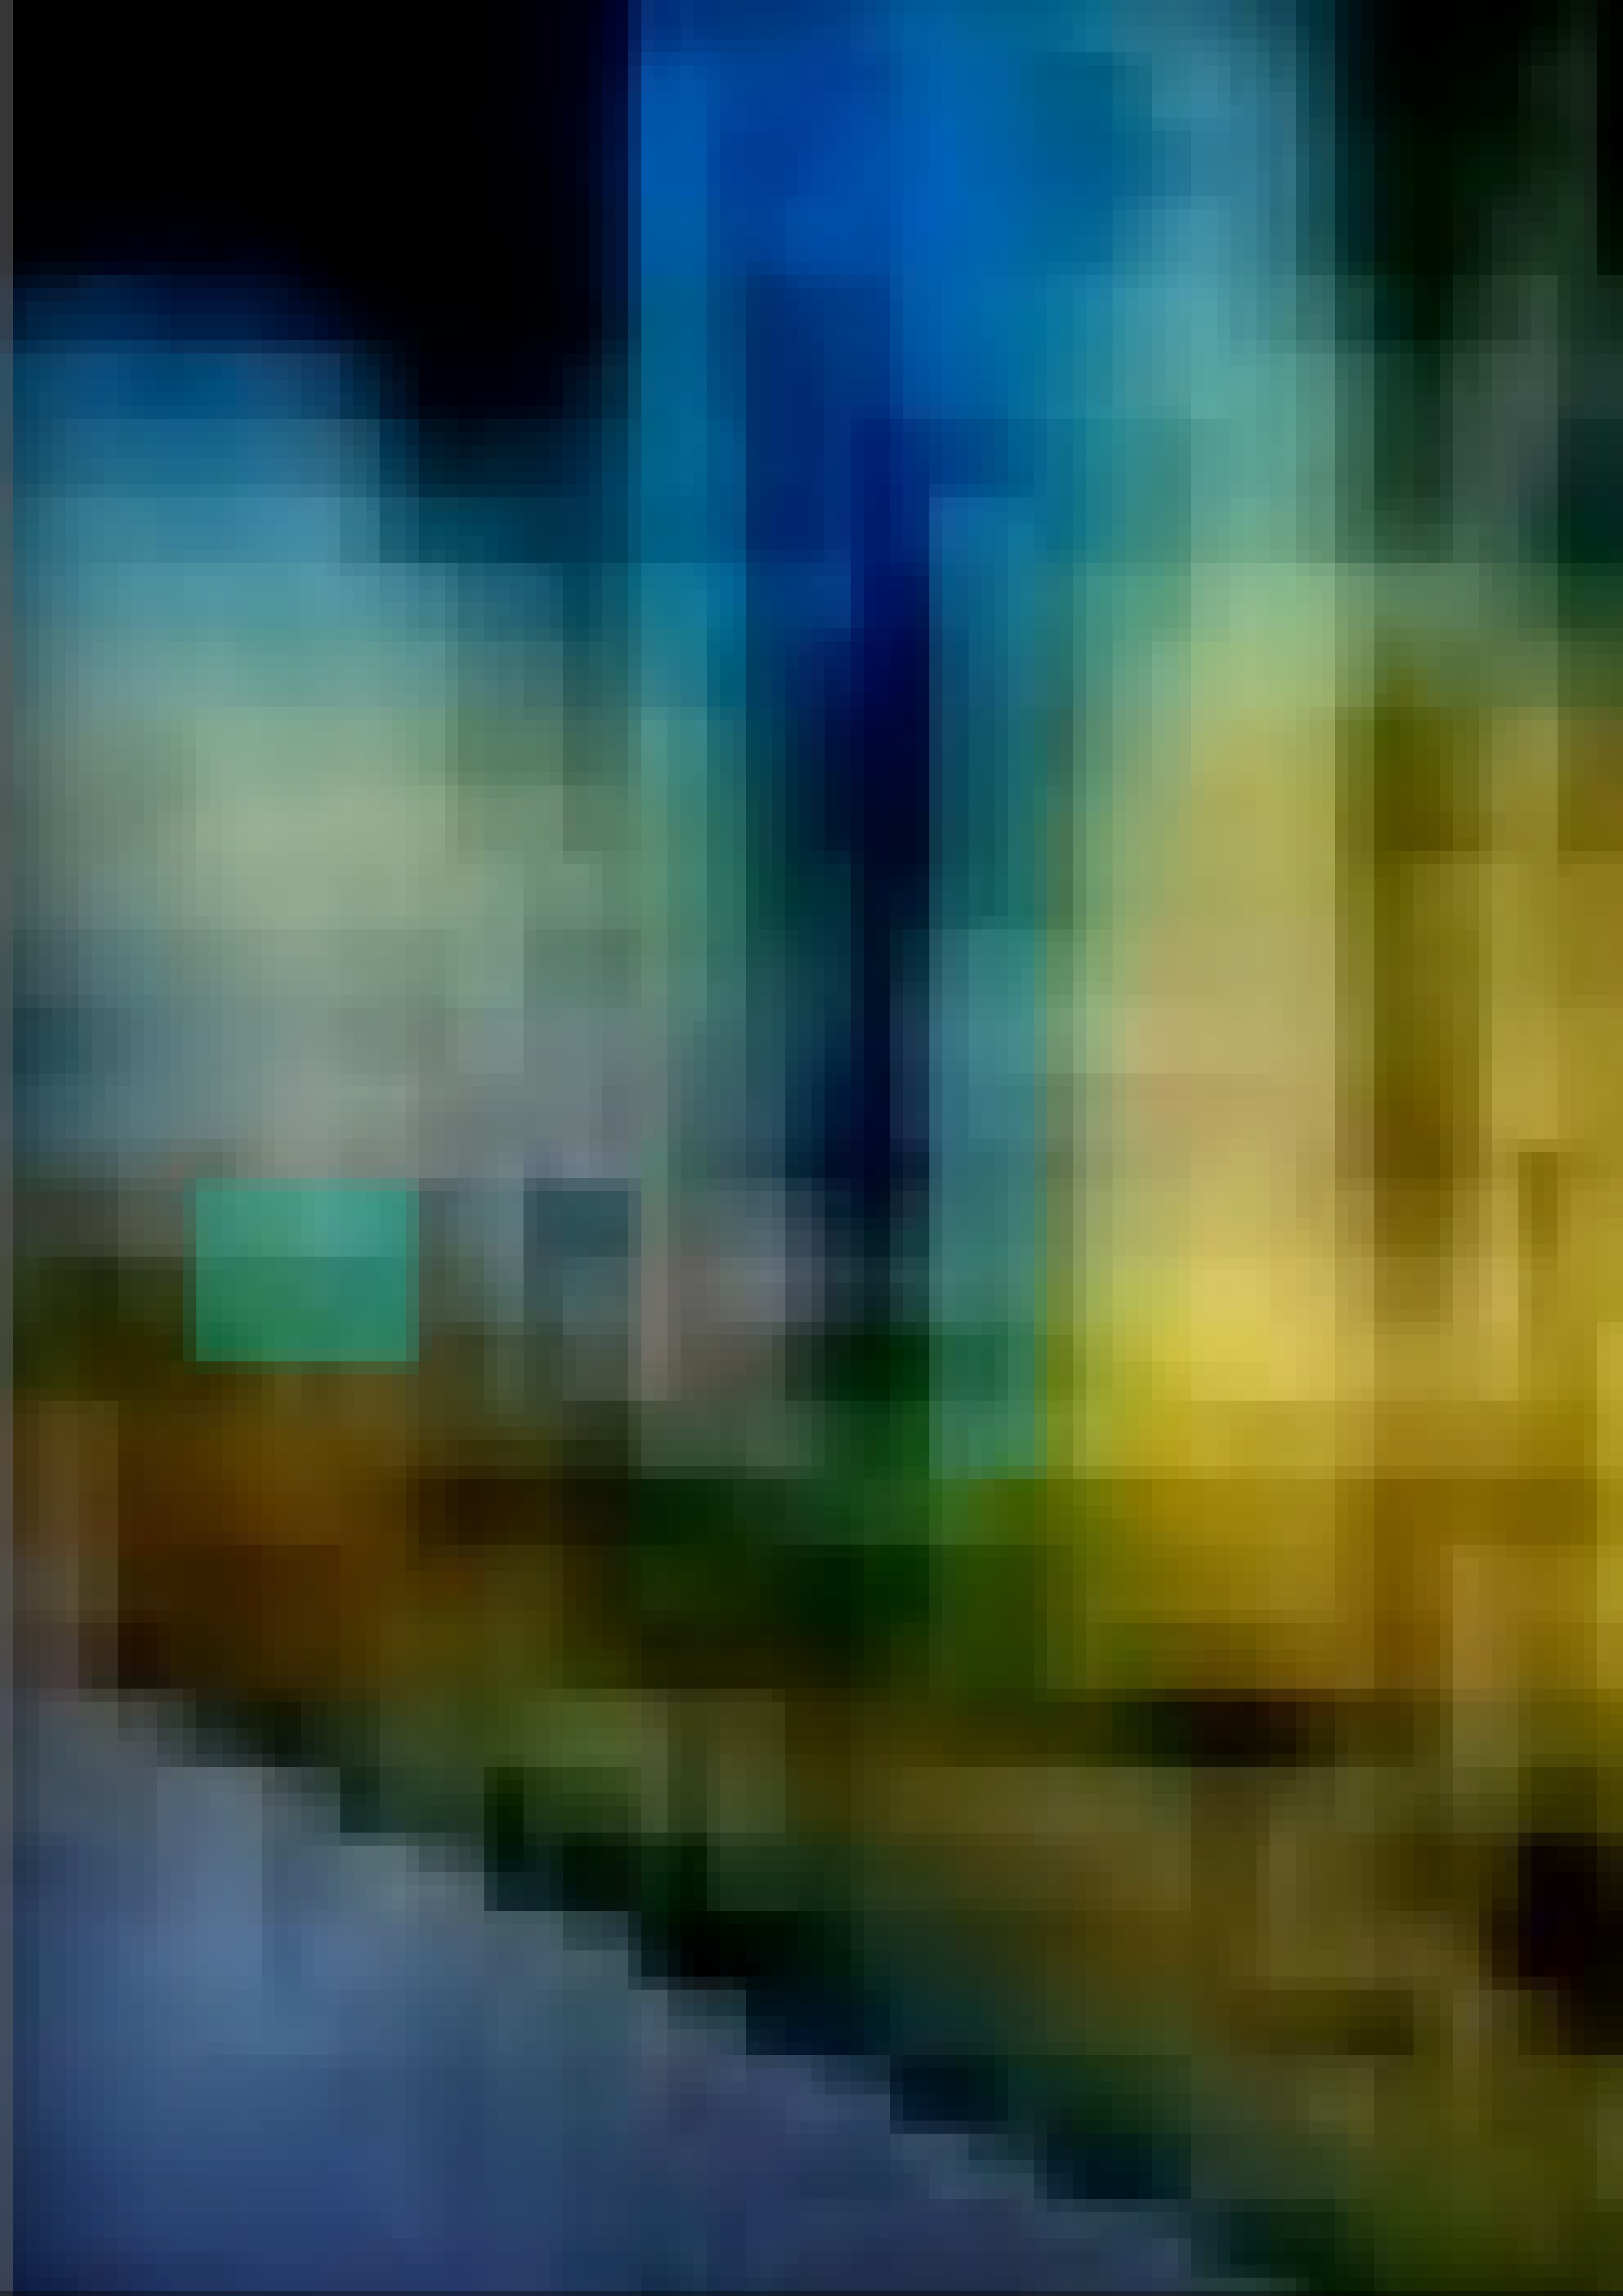
\includegraphics[width=0.4\textwidth]{images/FrontCover.png}
    \caption{Test caption of img}
    \figsource{Own graphic}
\end{figure}

\section{Motivation}
Using the representation a neural network has learned of an environment, to present the environment state to the player is a nearly unexplored avenue.
In this work I explore one way neural networks can be used in interactive experiences. I use the output of a neural network, that renders a camera at a position in an environment based on a learned internal representation, as the main information stream presented to the player.

\section{Scope}
During the bachelor project the following items where developed:

\begin{itemize}
\item{Data generation environment}
\item{Data processing pipeline}
\item{Scene rendering neural network model and training pipeline}
\item{System to send network output in Unity}
\item{Merging of network output with unity rendered objects}
\item{Several exploratory prototypes}
\item{One extended Prototype (Maze game)}
\end{itemize}
